\section{Data}

\subsection{Raw Data}

We use play-by-play from basketball referenece

% TODO: add citations
Downloaded from Kaggle [citation], scraped using [citation].

We clean and aggregate the data. One-hot encode columns corresponding to game events.

For example, col for jump shot, hook shot, dunk current score for each team, time left, etc.

Full list of columns given in \autoref{fig:list-of-columns}.

This data is fed into the neural network described in the next section.

\begin{figure}
	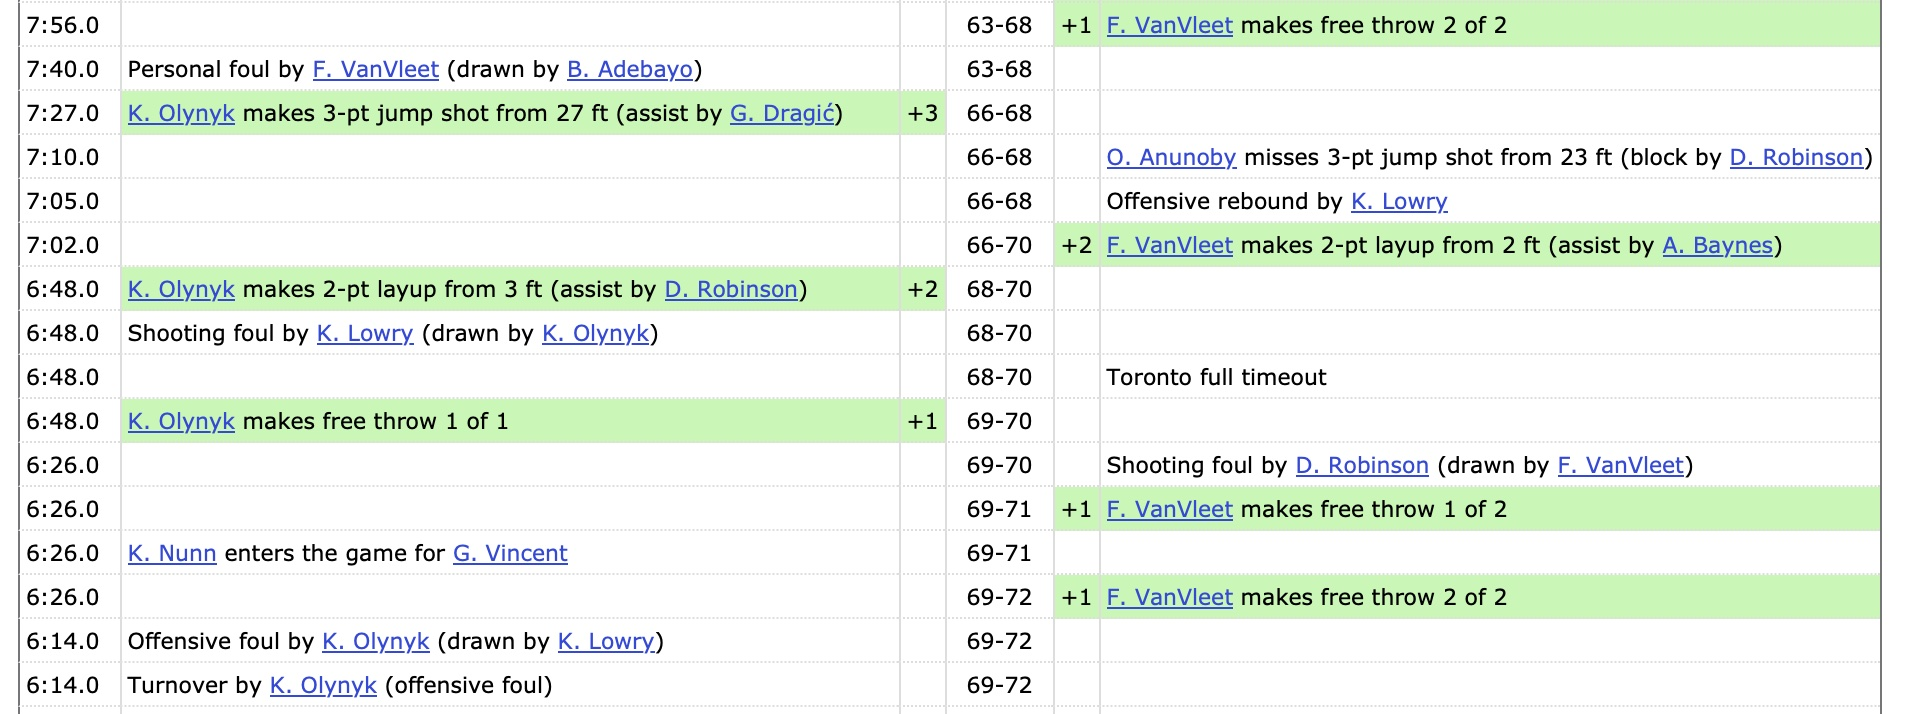
\includegraphics[width = .8 \textwidth]{figures/bbref-pbp.jpg}
	\caption{Example play-by-play data as seen on BasetballReference.com.}
\end{figure}

\begin{figure}
	% TODO: make this table
	\caption{The full list of the 69 columns in our data set.}
\end{figure}

\begin{figure}
	% TODO: make histogram 
	\caption{Histogram of the number of events per game.}
\end{figure}

\begin{figure}
	% TODO: make bar chart and/or table
	\caption{Number of events per event type.}
\end{figure}
